The Earth stands at a critical juncture in its history, where the consequences of human activity on the environment have reached a crossroads of global significance. Climate change, driven primarily by the relentless emission of greenhouse gases, has manifested itself in increasingly severe weather patterns, rising sea levels, and ecological disruptions. The urgency of the situation cannot be overstated, as nations grapple with the complex challenge of reducing carbon dioxide (CO$_2$) emissions to mitigate the impending climate crisis \cite{solomon2009irreversible,noaa-co2,world2016ambient}. 

The dire need for sustainable energy solutions has never been more evident. Various sectors of the economy are challenged to reduce their carbon footprint in order to restrict their impact on climate change. The transport sector was responsible for 23\% of global emissions from fuel combustion in 2021 and emerges as a critical contributor to the climate change predicament \cite{iea-transport}. 

\begin{figure}[h]
    \centering
    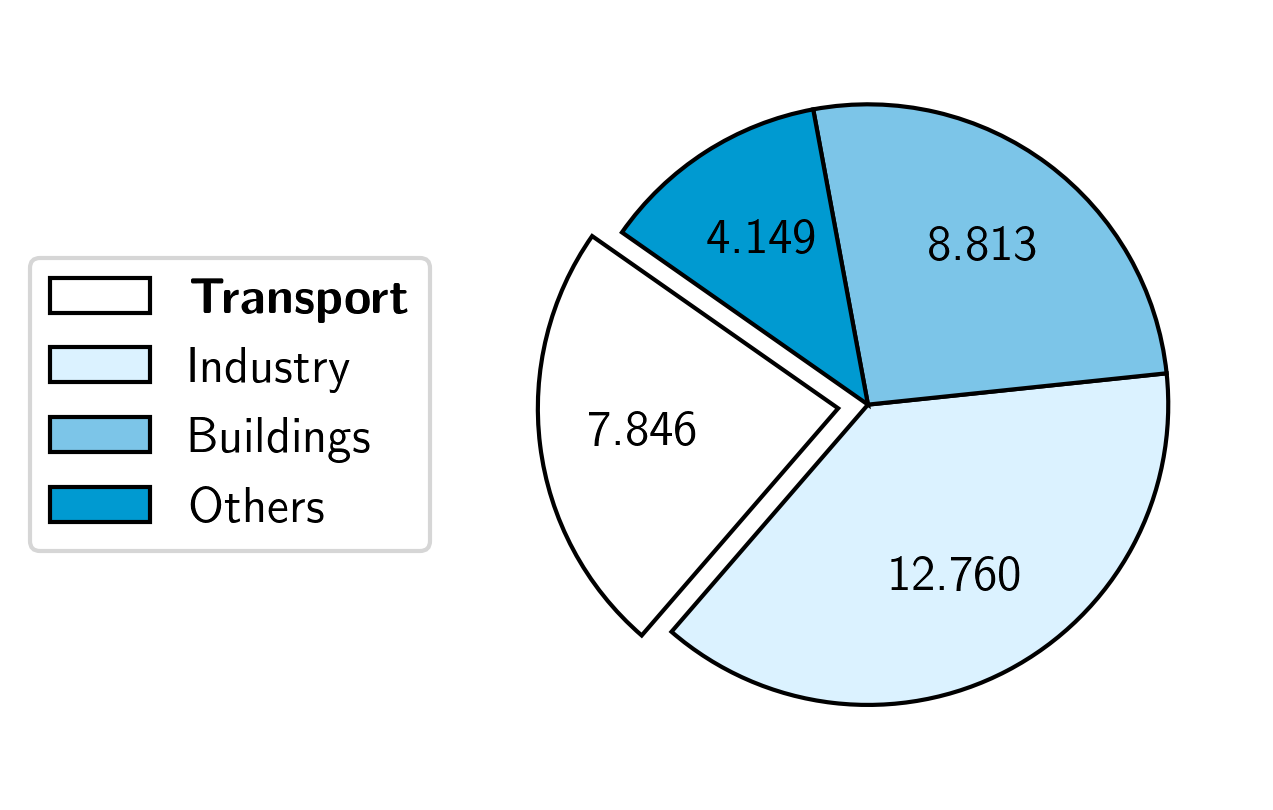
\includegraphics[width=0.65\textwidth]{Images/Chapter1/iea-transport2.png}
    \caption[2021 Global CO$_2$ emissions from fuel combustion by sector]{2021 Global CO$_2$ emissions from fuel combustion by sector [$\text{GtCO}_2$]. Source: IEA (2023) \cite{iea-transport}.}
    \label{fig:iea-transport}
\end{figure}

As societies evolve and the global population continues to grow, the demand for transportation, particularly in the form of automobiles and other fossil-fuel-reliant means, has risen dramatically. Innovative solutions are crucial to decouple the connection between personal mobility and CO$_2$ emissions. Electric vehicles (EVs) have emerged as a promising alternative to traditional internal combustion engine vehicles. They offer the potential to revolutionize the way we commute, significantly diminishing the transportation sector's contribution to carbon emissions. 

% \begin{figure}
%     \centering
%     
\includegraphics[width=0.7\textwidth]{Images/Chapter1/noaa-co2.png}
%     \caption{Trends in Atmospheric Carbon Dioxide. Source: NOAA (2023) \cite{noaa-co2}.}
%     \label{fig:noaa-co2}
% \end{figure}

At the heart of the electric vehicle industry's transformation lie lithium-ion batteries (LIBs). These energy storage devices have rapidly gained prominence as the primary means of powering EVs \cite{zubi2018lithium,stampatori2020li}. The suitability of LIBs for this role is driven by their impressive energy density, rechargeability, and relatively low environmental impact compared to conventional fossil fuels \cite{korthauer2018lithium}. As we explore the potential of lithium-ion batteries, it becomes evident that their development and adoption may hold the key to mitigating the environmental impact of the transportation sector. 

% This part has to be changed since it is copied from (Failure description: 890)
The shortcomings of LIBs are their narrow operational temperature range and charge-discharge rates. The capacity of the battery degrades faster if working at a high temperature, and the lifetime is shortened, too \cite{ma2018temperature,ning2003capacity}. When LIBs are subjected to conditions outside of their design window, they may fail through a rapid self-heating or thermal runaway, which may ignite the sorrounding materials \cite{palacin2016batteries}. 
% This part has to be changed since it is copied from (Matilda Thesis)
Hence, LIBs require meticolous safety testing in order to guarantee safe use in all usage frameworks. Safety tests must produce reliable parameters to enable satisfactory evaluation and classification of safe battery specifications. The consumer and industrial market demands safe, low-cost, high-power batteries produced with low environmental impact, using sustainable components that enable easy recycling \cite{doughty2012general}.

In the following sections the functioning of lithium-ion batteries is described, followed by a discussion of the safety and degradation issues that arise in LIBs.

\section{Overview}
\label{sec:overview}
A lithium-ion battery consists of two electrodes, an electrolyte, a separator, two current collectors and a metal casing. The positive and negative electrode materials are powders that are applied as coatings on current collector foils, resulting in composite electrodes. The ion-conducting electrolyte (containing a dissociated lithium conducting salt) is situated between two electrodes. The separator, an electrolyte-permeable membrane to electrically isolate the two electrodes, is also in that position.

\begin{figure}
    \centering
    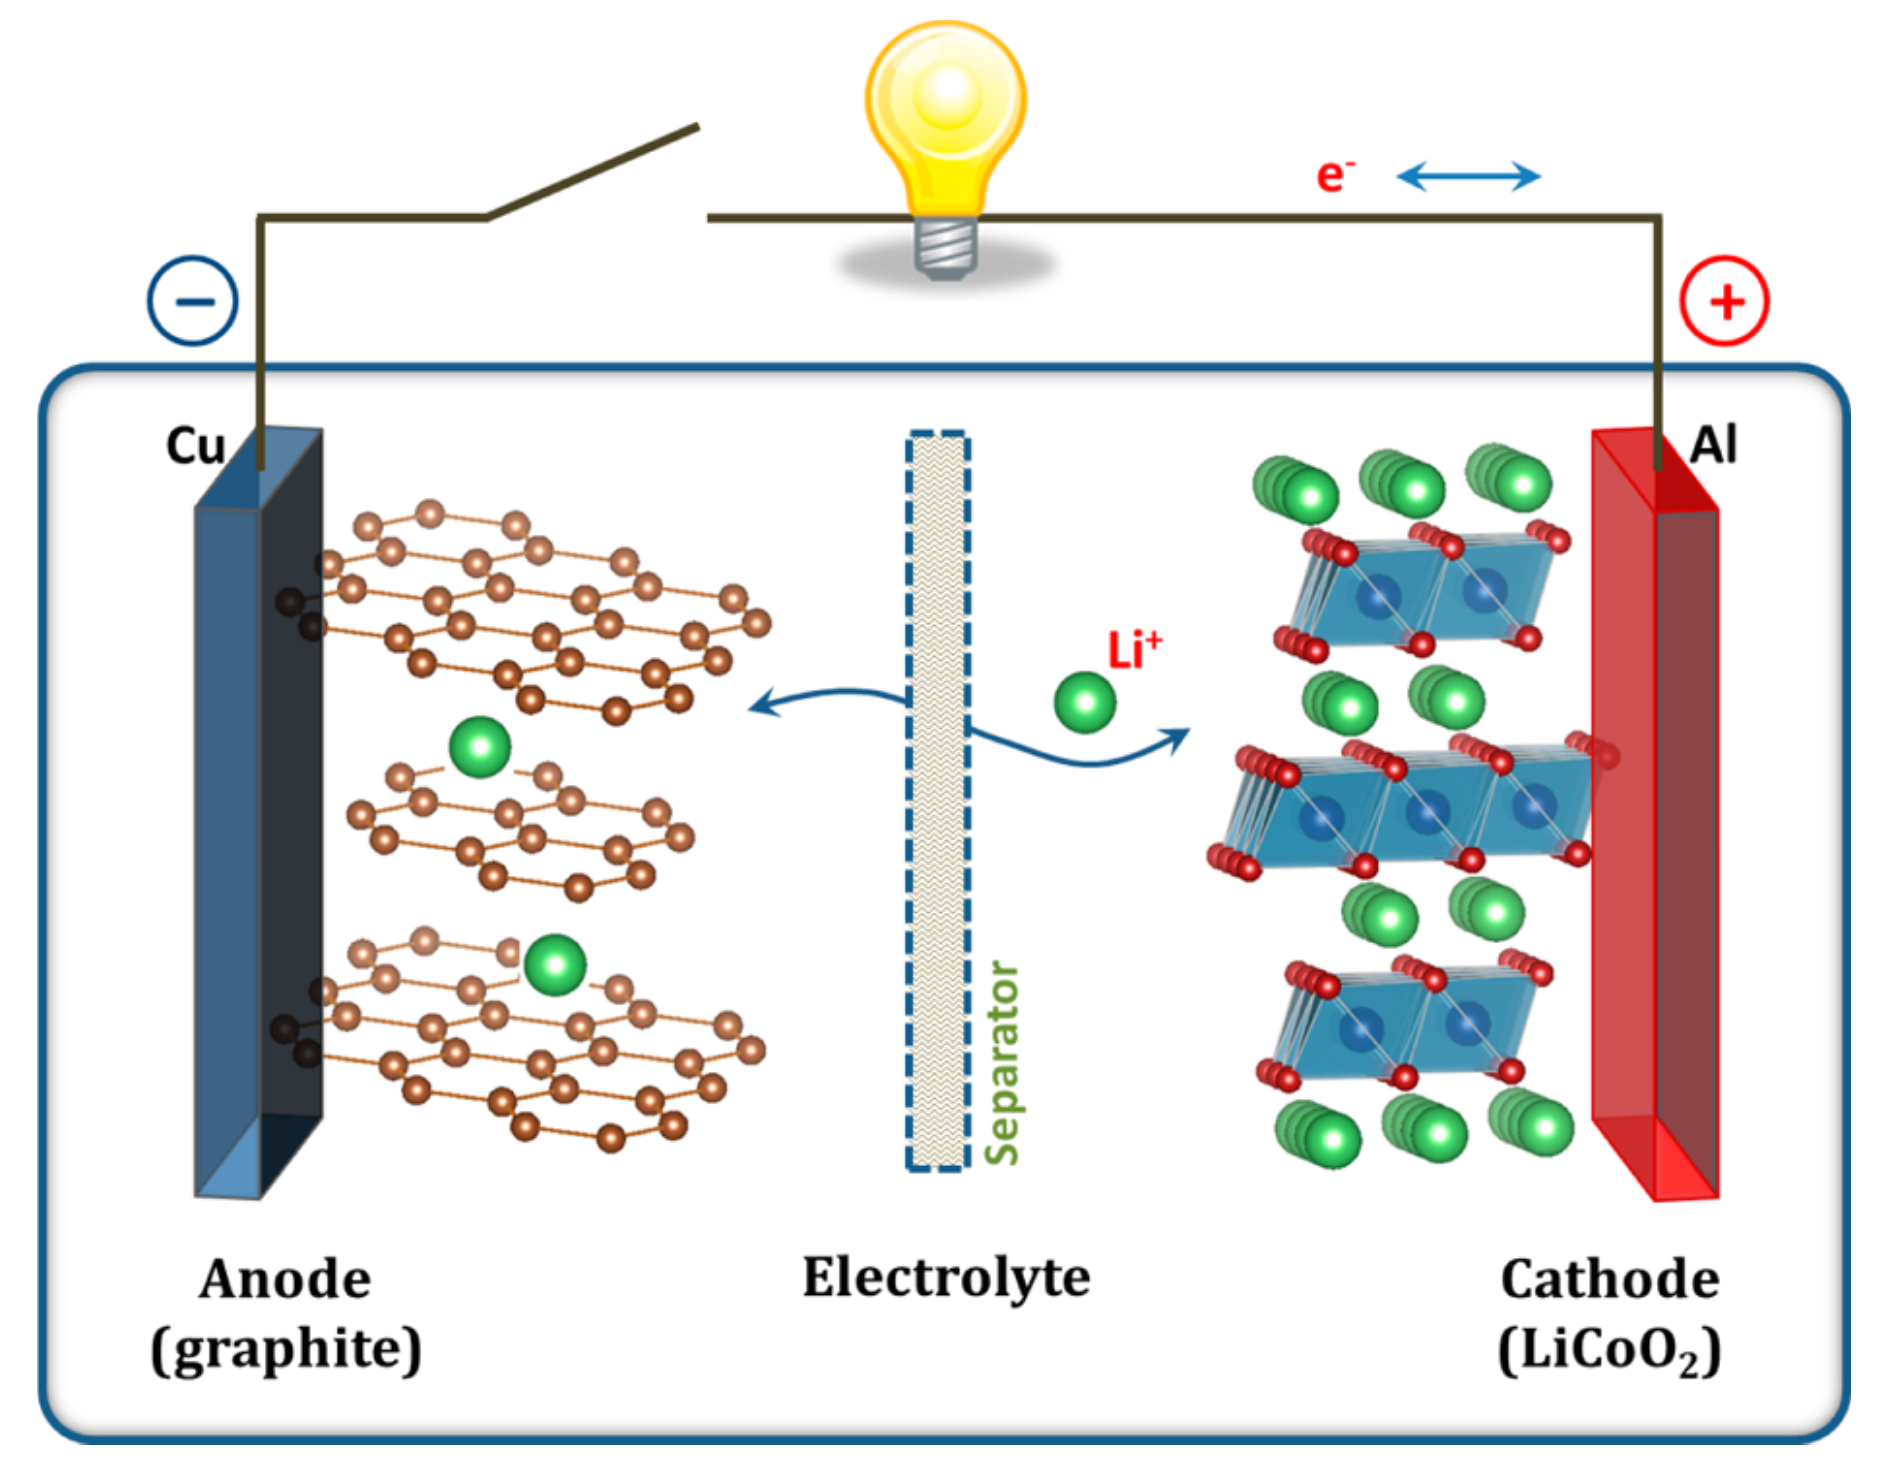
\includegraphics[width=0.8\textwidth]{Images/Chapter1/overview.png}
    \caption[Components of a traditional lithium-ion battery during discharging]{Components of a traditional lithium-ion battery during discharging. Source: Korthauer (2018) \cite{korthauer2018lithium}.}
    \label{fig:lib-overview}
\end{figure}

The electrolyte conducts the ionic component of the chemical reaction between the anode and the cathode, but it forces the electronic component to traverse an external circuit where it does work. Metallic current collectors deliver electronic current from/to the redox centers of the electrodes to/from the external circuit. These elements are used to produce cylindrical, prismatic and pouch cells. Depending on the application, a single battery cell is used or several cells are connected in series in a module. Also, a parallel connection is possible, dependent on the required capacity. Several connected modules form a battery system for auto-motive applications \cite{korthauer2018lithium,goodenough2013li}.

\subsection{Positive Electrode}
\label{sec:positive-electrode}
% See the book for articles to cite in these parts!
% This part has to be changed since it is copied from (Li-ion definitive book)
Lithium transition metal compounds are employed as positive electrode materials. These composites can develop mixed crystals over an ample composition range and can deintercalate lithium ions from the structure during the charging process. The traditional positive electrode material is lithiated cobalt oxide, LiCoO$_2$. It has a layered structure with alternating cobalt, oxygen, and lithium ion layers. During charging, lithium leaves the crystal (deintercalation); during discharging, it returns (intercalation). However, only 50\% of the lithium may be utilized. If more than half of the lithium leaves the crystal, the structure may collapse and liberate oxygen. This can cause thermal runaway, as oxygen is able to burn the electrolyte. 

For complete discharging, the reaction at the positive electrode is:
\begin{equation}
    \label{eq:positive-electrode}
    2\text{Li}_{0.5}\text{CoO}_2 + \text{Li}^+ + e^- \rightarrow 2\text{LiCoO}_2
\end{equation}
Thus for one mole (7 g) of active lithium, two moles (189 g) of Li$_{0.5}$CoO$_2$ are needed as host for lithium during discharge.

The use of cobalt oxide as positive electrode material is not safe. If it is kept “fully” charged as Li$_{0.5}$CoO$_2$, it reacts slowly with the electrolyte, thus losing performance. If it is slightly overcharged, there is a clear loss in capacity and service life. In case of severe overcharging, the cobalt oxide crystal collapses which can cause thermal runaway and fire. Overcharging easily happens, as there is no obvious voltage difference between normal charging and overcharging. Cobalt oxide is expensive, as cobalt ore is scarce. This problem is getting worse as the demand grows. Economics of scale do not apply here. Last but not least, cobalt is toxic.

The main commercial alternatives for cobalt oxide are listed in Table \ref{table:cathode-alternatives}. Each of the alternative materials solves some of the problems but they all are compromises. LMO is safer and very cheap but has a limited service life. NCM is safer and cheaper, but has a sloping discharge voltage. NCA is cheaper and lighter (more specific capacity, mAh/g) but it is hardly safer. LFP is very safe and slightly cheaper, but it gives 0.5 V lower voltage than cobalt oxide. At the moment, NCM and LFP seem to be the most promising candidates for large-scale batteries.

\begin{table}[H]
    \centering 
        \begin{tabular}{|c c c|}
        \hline
        \rowcolor{bluepoli!40}
        \textbf{Compound} & \textbf{Abbreviation} & \textbf{Chemical structure} \T\B \\
        \hline \hline
        Manganese oxide & LMO & LiMn$_2$O$_4$\T\B\\
        \hline
        Nickel manganese cobalt oxide & NCM & LiNi$_{1/3}$Mn$_{1/3}$Co$_{1/3}$O$_2$\T\B\\
        \hline
        Nickel cobalt aluminum oxide & NCA & LiNi$_{0.8}$Co$_{0.15}$Al$_{0.15}$O$_2$\T\B\\
        \hline
        Iron phosphate & LFP & LiFePO$_4$\T\B\\
        \hline
        \end{tabular}
        \\[10pt]
        \caption[Commercial alternatives for cobalt oxide]{Commercial alternatives for cobalt oxide. Source: Korthauer (2018) \cite{korthauer2018lithium}.}
        \label{table:cathode-alternatives}
\end{table}

\subsection{Negative Electrode}
\label{sec:negative-electrode}
% See the book for articles to cite in these parts!
% This part has to be changed since it is copied from (Li-ion definitive book)
By far the most common negative electrode material is graphitic carbon. It has carbon atoms in parallel graphene layers. During charging, the lithium ions are intercalated into the graphite, between its layers. During discharging, lithium leaves the graphite. Unlike cobalt oxide, graphite is stable even without lithium, so it can be almost completely discharged. For complete discharging, the reaction at the negative electrode is:
\begin{equation}
    \label{eq:negative-electrode}
    \text{LiC}_6 \rightarrow \text{Li}^+ + e^- + 6\text{C}
\end{equation}
Thus for one mole (7 g) of active lithium, there are six moles (72 g) of carbon that act as host for the lithium during charging.

Graphite as negative electrode is not safe either. For graphite, the lithium intercalation potential is only about 80 mV more positive than the lithium metal plating potential. Even a small design failure or charging error causes deposition of metallic lithium on the electrode surface. Small amounts of metallic lithium increase the reactivity of the graphite surface, thus consuming electrolyte in secondary reactions. Large amounts of deposited lithium metal can grow as metallic peaks, “dendrites”, that short-circuit the negative and positive electrodes. This might cause excess heating and ignite the electrolyte resulting in a fire.

The potential of lithiated graphite is far beyond the stability window of the common electrolytes. During the first charging of the battery, graphite reacts with the electrolyte, building a protective layer on the graphite surface. This solid electrolyte interface (SEI) layer should prevent further secondary reactions. However, some secondary reactions take place throughout the lifetime of the battery, reducing its cyclic and calendar life.
Some commercial alternatives for graphite exist. Soft and hard carbons are used due to their slightly more positive intercalation potentials. This means less risk of lithium metal deposition and a possibility of faster charging.
However, the energy density is considerably lower when these materials are used. Lithium titanate is a very safe negative electrode material with an amazingly long service life, but the 1.4 V lower cell voltage limits the use of lithium titanate to very few applications. The newest commercial alternative, silicon, gives a formidable energy density, but low stability limits its service life.

Graphite is cheap and lightweight, especially when compared to cobalt oxide. Therefore, it can be expected that graphite retains its position as standard negative electrode material in the near future.

\subsection{Electrolyte}
\label{sec:electrolyte}
% This part has to be changed since it is copied from (Li-ion definitive book)
Electrolytes are an essential component of a lithium-ion battery. The requirement profile of the perfect electrolyte is manifold and encompasses, among other things:
\begin{itemize}
    \item[--] high conductivity across a wide temperature range ($-40^\circ$C to $80^\circ$C);
    \item[--] cycling stability over several thousands of cycles;
    \item[--] chemical/electrochemical compatibility with the electrode and inactive materials;
    \item[--] risk minimization of thermal runaway and other hazardous reactions during battery operation;
    \item[--] ecological sustainability;
    \item[--] balance between cost and performance.
\end{itemize}
The tool box for each electrolyte for lithium-ion batteries consists of three classes of materials: conducting salt, organic aprotic solvents, and additives. It is the combination of these components which largely determines the physico-chemical and electrochemical characteristics of the electrolyte and contributes to fulfilling the above-mentioned objectives. 

At the same time, the electrolyte is not an independent component of the cell. It needs to be chosen in dependence on the materials for the anode and the cathode side. That, in turn, calls for close collaboration between the electrolyte manufacturer and the cell and battery developers \cite{korthauer2018lithium}.

\subsubsection{Solvents}
\label{sec:solvents}
In lithium-ion batteries highly reductive materials are used for the negative electrode and highly oxidizing components for the positive electrode. This is the reason why solvents with an active acidic proton are unsuitable. This would immediately lead to a development of hydrogen. The same reason excludes water as a solvent. Other mandatory requirements for the solvent are:
\begin{itemize}
    \item[--] high permittivity $\epsilon$: the solvent must be able to dissolve lithium salts in a sufficiently high concentration;
    \item[--] low viscosity $\eta$: unimpeded ion transport in the electrolyte is needed, especially at low temperatures and for high-voltage applications;
    \item[--] inertia towards all other cell components in all operating conditions;
    \item[--] low melting point $T_m$ and high boiling point $T_b$: the electrolyte must be liquid over the entire operating temperature range of the battery;
    \item[--] low toxicity and low cost.
\end{itemize}

Two classes of organic solvents that are simultaneously aprotic and highly polar have gained recognition as suitable materials for lithium-ion batteries: ethers and esters, including organic carbonates.

Ether-containing electrolytes for the most part exhibit a low viscosity and therefore a very high conductivity. But their electrochemical stability is restricted and they are already oxidized at potentials around 4 V vs. Li/Li$^+$. With the introduction of 4-V transition metal oxides as positive electrode materials, ethers have therefore disappeared as solvents for high-energy lithium-ion batteries.

Esters, especially organic diesters of carboxylic acid (so-called carbonates), are current state of the art. In general, the following are employed: blends of cyclic carbonates (e.g., ethylene carbonate [EC] and, to some extent, propylene carbonate [PC]) that exhibit a high dipole moment at moderate viscosity. Also, open-chain carbonates (dimethyl carbonate [DMC], diethyl carbonate [DEC], and ethyl methyl carbonate [EMC]) are used, which exhibit a moderate dipole moment at low viscosity \cite{xu2004nonaqueous,aurbach1995study,song1999review}.

\begin{table}[H]
    \centering
        \begin{footnotesize}
            \begin{tabular}{|p{16mm} p{24mm} p{20mm} p{20mm} p{20mm} p{24mm}|}
                \hline
                \rowcolor{bluepoli!40}
                \textbf{Solvency} & \textbf{Structure} & \textbf{Melting point} [$^\circ$C] & \textbf{Boiling point} [$^\circ$C] & \textbf{Viscosity} (25 $^\circ$C) [cP] & \textbf{Permittivity} (25 $^\circ$C) \T\B \\
                \hline \hline
                EC & \includegraphics*[width=24mm]{Images/Chapter1/EC.png} & 36 & 247-249 & 1.9 (40 $^\circ$C) & 90 (40 $^\circ$C)\T\B\\
                \hline
                PC & \includegraphics*[width=24mm]{Images/Chapter1/PC.png} & $-$48 & 242 & 2.53 & 65\T\B\\
                \hline
                DMC & \includegraphics*[width=24mm]{Images/Chapter1/DMC.png} & 2$-$4 & 90 & 0.59 & 3.1\T\B\\
                \hline
                DEC & \includegraphics*[width=24mm]{Images/Chapter1/DEC.png} & $-$43 & 125-129 & 0.75 & 2.8\T\B\\
                \hline
                EMC & \includegraphics*[width=24mm]{Images/Chapter1/EMC.png} & $-$55 & 108 & 0.65 & 3.0\T\B\\
                \hline
                \end{tabular}
                \\[10pt]
                \caption[Psycho-chemical characteristics of selected battery solvents]{Psycho-chemical characteristics of selected battery solvents. Source: Korthauer (2018) \cite{korthauer2018lithium}.}
                \label{table:solvents}
        \end{footnotesize}
\end{table}

\subsubsection{Conducting Salts}
\label{sec:conducting-salts}
The electrolyte provides for the lithium ion transport between the electrodes. Therefore, a suitable lithium salt must provide maximum solubility and complete dissociation in aprotic solvents to ensure a high lithium-ion mobility. Very high electrochemical anion stability is also needed, in addition to high chemical stability in respect to the solvent. This requirement profile leads to mostly complex anions in which the negative charge is distributed to a high extent across the anions. This reduced charge density in turn causes a low attraction between the anion and the lithium cation, which determines the free movement of the cation and is therefore necessary for a high mobility.

In terms of the compounds possible in principle, lithium hexafluorophosphate (LiPF$_6$) plays a special role. Nowadays, commercial lithium-ion batteries are almost exclusively equipped with LiPF$_6$. This is on the one hand not by reason of a single outstanding characteristic, but of an unparalleled unique combination of characteristics. And on the other hand it is based on the willingness to accept individual disadvantages.

Having a conductivity of 8 to 12 mS/cm (room temperature, 1 mol/l), LiPF$_6$ forms highly conductive electrolytes in blends of organic carbonates. These electrolytes are, in addition, electrochemically stable up to almost 5 V vs. Li/Li$^+$. LiPF$_6$ is one of the few conducting salts that very effectively prevent the corrosion of the aluminum current collector of the positive electrode at potentials above 3 V vs. Li/Li$^+$. Production process, quality, and purity, crucial for a battery's performance, have been improved over the course of the years: high-purity LiPF$_6$ has been available on an industrial scale for more than 30 years. Today's lithium-ion technology has been developed based on this conductive salt.

The limited chemical and thermal stability of LiPF$_6$ are its main disadvantages. In its pure form it very slowly disintegrates into traces of lithium fluoride (LiF) and phosphorous pentafluoride (PF$_5$), creating an equilibrium. High temperatures promote this process.
\begin{equation}
    \label{eq:lipf6-dissociation}
    \text{LiPF}_6 \rightleftharpoons \text{LiF} + \text{PF}_5
\end{equation}

Lithium-bis(trifluoro- methylsulfonyl)imide (LiTFSI) and lithium-bis(fluorosulfonyl)imide (LiFSI) have increasingly been introduced into the market as alternatives to LiPF$_6$. They are characterized by a high thermal stability, however they are not as electrochemically stable as LiPF$_6$ and are not as effective in preventing corrosion of the aluminum current collector. In addition, they are more expensive and less soluble in organic solvents. LiTFSI and LiFSI are therefore used in combination with LiPF$_6$ \cite{xu2004nonaqueous}.

\subsubsection{Additives}
\label{sec:additives}
Additives mainly are employed to optimize the so-called solid electrolyte interface (SEI), the boundary surface between the negative electrode and the electrolyte. The SEI significantly influences service life and performance of the lithium-ion cell.
Lithium ions do not exist in the form of “naked” cations in organic polar solvents, but rather as complex cation solvent adducts. This so-called solvate complex is many times larger than the naked lithium ion.
Solvated lithium ions penetrate into the outer structures of the graphite anode during charging of the lithium-ion cell. The solvents (and in part also the anion of the lithium salt) degrade owing to the extremely reductive conditions and form hardly soluble precipitates. They accumulate on the electrode and in the outer structures of the graphite and form the layer that is called SEI.
This layer is permeable for lithium ions. At the same time it is electrically isolating and prevents the direct contact of electrode and solvent, a characteristic that prevents further degradation of the solvent. All carbonates employed in lithium-ion batteries nowadays form an SEI. The quality and composition of the layer, however, strongly depend on the chosen solvent combination.

\begin{figure}[ht]
    \centering
    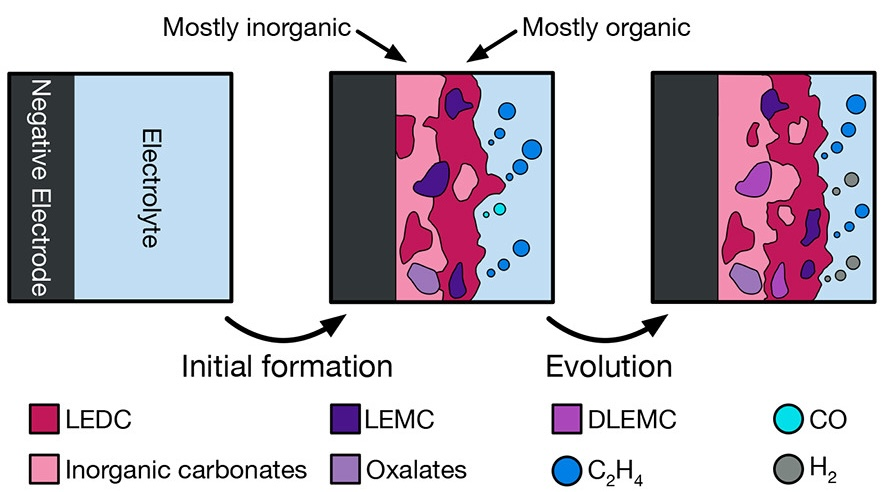
\includegraphics[width=0.65\textwidth]{Images/Chapter1/sei.jpeg}
    \caption[Mechanistic model of the SEI]{Mechanistic model of the SEI. Source: Spotte-Smith (2022) \cite{spotte2022toward}.}
    \label{fig:sei}
\end{figure}

The SEI's structure and characteristics might be influenced significantly by the additives. The SEI additives must be more reactive electrochemically than all other components of the electrolyte in order for the SEI to be reduced during the first charging cycle of the lithium-ion cell before the solvents. This way, an SEI is formed before the solvents react.
The best-known example of this class of additives is vinylene carbonate. It is used in almost every commercial lithium-ion cell and leads to a significant improvement of the cycling stability. It becomes effective during the first charging and discharging cycles of the lithium-ion cell \cite{xu2004nonaqueous}.

\subsection{Separator}
\label{sec:separator}
Battery separators are flat materials situated between the positive and negative electrodes of a battery cell. Their function is to prevent physical contact and, there- fore, short circuits. At the same time, they must enable ions to be transported as freely as possible within the electrolyte between the electrodes. This is essential for charge equalization and the electrochemical cell to work. To achieve this, separators are usually porous flat designs filled with an electrolyte.

\begin{table}[H]
    \centering
        \begin{footnotesize}
            \begin{tabular}{|p{18mm} p{132mm}|}
                \hline
                \rowcolor{bluepoli!40}
                \textbf{Property} & \textbf{Description}\T\B \\
                \hline \hline
                \textbf{Thickness} & The separators of consumer application lithium-ion cells are relatively thin. They have a thickness of less than $\mu$m. However, thicker separators (up to 40 $\mu$m) are used for the production of large-size lithium-ion cells. These have considerably higher mechanical stability and puncture resistance.\T\B\\
                \hline
                \textbf{Porosity} & Standard separators for lithium-ion cells have a porosity of around 40\%. Controlling the porosity is of great importance in separator manufacturing and immensely influences the porosity of the end product. In addition, high porosity enables a larger electrolyte reservoir. Non-uniform porosity, on the other hand, leads to non-uniform current densities which result in the electrodes aging more rapidly.\T\B\\
                \hline
                \textbf{Pore size} & The pores must be small enough to prevent an electrical connection caused by loose electrode particles. Also, they need to prevent dendrite growth in the lithium-ion cell. Separators with a thickness of < 25 $\mu$m are assumed to have an average pore size in the submicron range. The pore size distribution in battery separators must be as homogeneous as possible, as is the case for requirements related to porosity. This enables a uniform current density and thus uniform aging of the cell.\T\B\\
                \hline
                \textbf{Chemical stability} & The separators must be chemically and electrochemically stable in both the battery and its electrolyte. In particular, the development of high-voltage materials has given rise to new requirements for separators.\T\B\\
                \hline
                \end{tabular}
                \\[10pt]
                \caption[Separators essential properties]{Separators essential properties. Source: Korthauer (2018) \cite{korthauer2018lithium}.}
                \label{table:separator-properties}
        \end{footnotesize}
\end{table}

In lithium-ion cells, battery separators are mostly based on polyolefins into which submicronsized holes are introduced by means of a physical process. These battery separators can be divided into two classes based on their production process: microporous polyolefin membranes and wet membranes.
Resulting from their chemical and physical compositions, these two separator classes exhibit in part extremely different characteristics.

Microporous polyolefin membranes exhibit a thickness up to 12 to 40 $\mu$m, a maximum pore size of < 0.5 $\mu$m, and a high tensile strength. The low thickness positively influences the energy density of the battery. The pore distribution protects them against dendrite formation quite well. The disadvantages of these membranes are their low porosity (around 40\%), low melting point (around 160 $^\circ$C for PE), and very high shrinkage (20\% at 120 $^\circ$C/10 min) at higher temperatures. This is increasingly true for larger cells because they dissipate heat poorly. If the separator loses its structure, there will be contact between the electrodes and thus a reaction of the electrode materials. This can cause the battery to explode.

Wet membranes have a thickness of up to 25 $\mu$m, uniform pore distribution with short distances (< 1 $\mu$m), and high tensile strength. The low thickness positively influences the energy density of the battery. The short pore distances effectively prevent dendrites from forming. As with the microporous polyolefin membranes, the tensile strength is beneficial for producing cylindrical cells. The disadvantages of these membranes are their low melting point (around 135 $^\circ$C) and very high shrinkage (7 to 30\% at 120 $^\circ$C/10 min) \cite{arora2004battery,bladwin2009review}.

\begin{figure}[ht]
    \centering
    \subfloat[Microporous polyolefin membrane.\label{fig:polyolefin-membrane}]{
        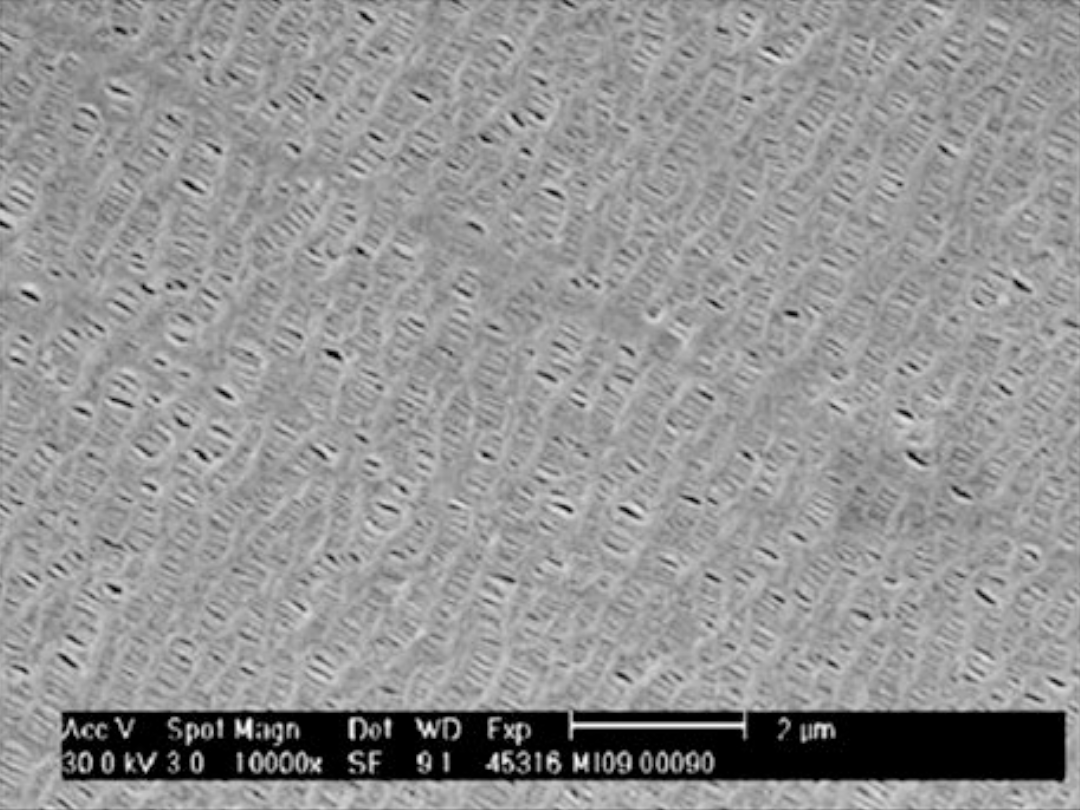
\includegraphics[scale=0.38]{Images/Chapter1/polyolefin.png}
    }
    \quad
    \subfloat[Wet membrane.\label{fig:wet-membrane}]{
        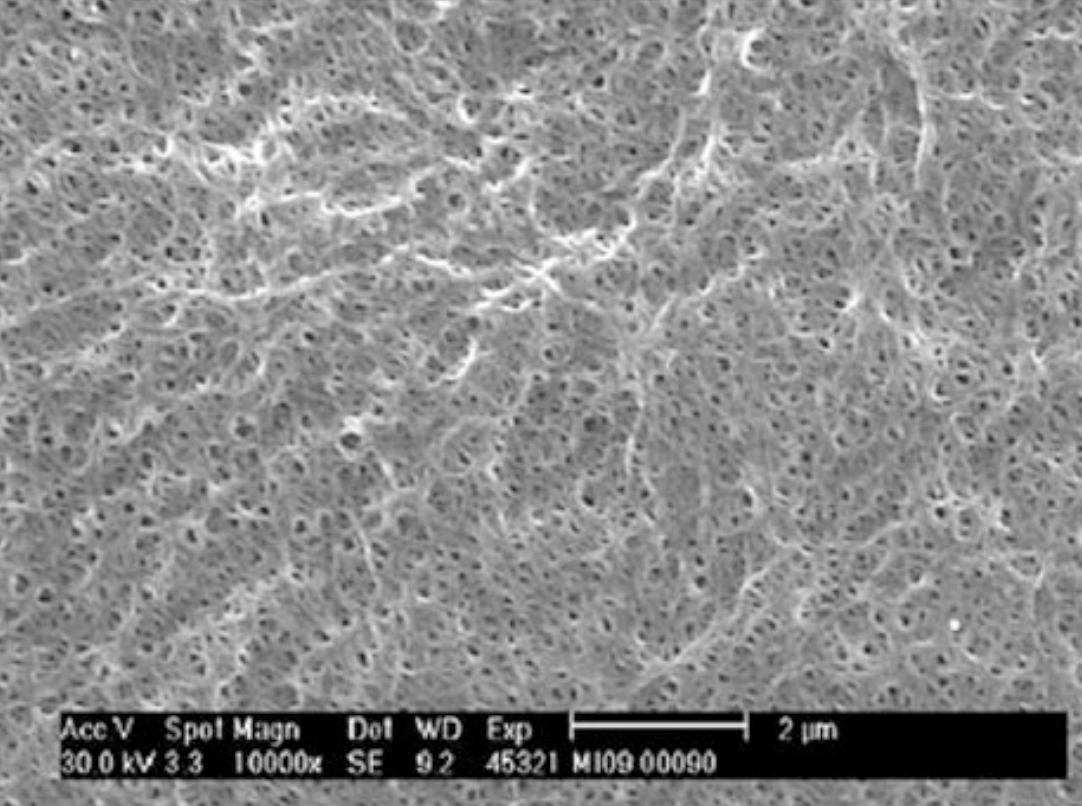
\includegraphics[scale=0.38]{Images/Chapter1/wet.png}
    }
    \caption[Scanning electron microscopic pictures of separators]{Scanning electron microscopic pictures of a microporous polyolefin membrane and a wet membrane. The samples were metallized with gold to achieve a higher resolution. Source: Korthauer (2018) \cite{korthauer2018lithium}.}
    \label{fig:separators}
\end{figure}

\subsection{Current Collectors}
\label{sec:current-collectors}
By enabling conduction of electrons between the electrodes and the battery terminals, the current collectors greatly impact the performance of the battery. The current collectors are viewed as un-active components of the cell but can however make up 15\% of the cell weight. Properties such as electrochemical stability, electrical conductivity, mechanical strength, density, sustainability and cost has to be thoroughly evaluated. In conventional lithium-ion batteries the most commonly used materials are copper and aluminum foil for the negative and the positive electrode respectively. A high electrical conductivity is required for efficient transportation of electrons through the external circuit of the battery. 

As for any other component of the battery, the ability of the current collectors to sustain in an electrochemical environment and not to undergo undesired reactions is vital. Furthermore, it is crucial to maintain a satisfying adhesion between the current collectors and the electrodes; to achieve this, polymeric binders such as PVDF are commonly used. Both aluminum and copper show high electrical conductivity and valuable mechanical properties. The low density of aluminum (2.70 g$\cdot$cm$^{-3}$) contributes to an increase in gravimetric energy density, while copper on the contrary has a high density of 8.96 g$\cdot$cm$^{-3}$. Consequently, for the case of the copper foil there is a trade-off between high electrical conductivity and thickness. In terms of heat generation, the current collectors act as efficient heat dissipators due to their high thermal conductivity and play an important role in the events leading up to a thermal runaway \cite{zhu2021review}.

\subsection{Cell Geometries and Designs}
\label{sec:cell-geometries-designs}
All of today’s lithium-ion cells exhibit metal-based housing and packaging material. One reason is that it prevents the entry of moisture into the cell, which would initiate a hydrolysis of the conducting salt LiPF6 into hydrogen fluoride (HF). Another is the prevention of loss of solvent by means of diffusion from the cell. Only metal is able to fulfill these tasks. A housing made of pure plastics is not suitable because no plastic (not even polypropylene) is completely moisture leaktight. The solid metallic housings (hardcase) are typically made of aluminum or stainless steel.

\begin{figure}[ht]
    \centering
    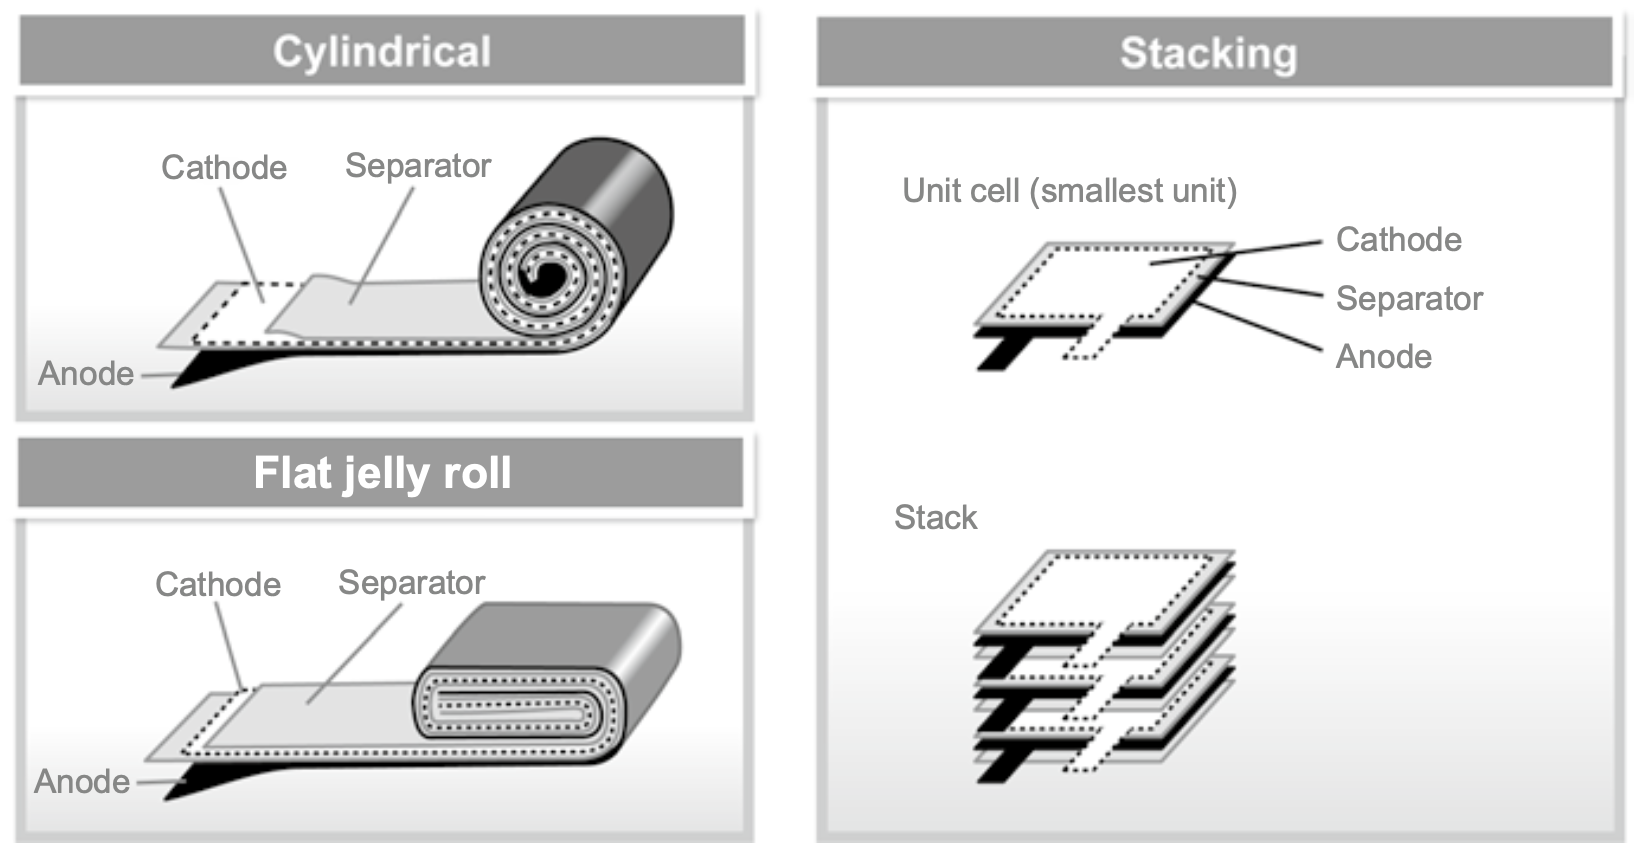
\includegraphics[width=0.8\textwidth]{Images/Chapter1/geometries.png}
    \caption[Inner structure of lithium-ion cells]{Inner structure of lithium-ion cells. Source: Korthauer (2018) \cite{korthauer2018lithium}.}
    \label{fig:geometries}
\end{figure}

\section{Safety and Degradation}
\label{sec:safety-degradation}

